\chapter{Analysis and Discussion}
\label{ch:discussion}

%-------------------------------------------------------

\section{Failure analysis}
\label{sec:failures}

Every strict top-1 failure of the single-card experiment was assigned exactly one cause by fixed rules (\texttt{cardrec/failure\_analysis.py}), checked in this order: \emph{localisation} (outline IoU $<0.5$), \emph{rectification} ($0.5 \leq$ IoU $<0.8$), \emph{upside down} (only for rotation-sensitive methods, when the true rotation lies outside the window that the warp returns upright), \emph{same artwork} (the prediction is a reprint), \emph{lookalike} (the prediction has the same name), \emph{heavy distortion} (severity 4--5 and none of the above) and \emph{other}. Because the first matching rule wins, the counts show the earliest stage at which a query went wrong, not every problem it had. Table~\ref{tab:failures} and Figure~\ref{fig:failure-causes} show the result; Figure~\ref{fig:failure-examples} shows one example per cause.

\begin{table}[htbp]\centering\small
\caption[Failure causes]{Cause of every strict top-1 failure on the synthetic single-card queries (all finished severities pooled; recomputed from the current logs). Each failure gets the first cause that applies, in the column order.}\label{tab:failures}
\begin{tabular}{@{}lrrrrrrrr@{}}
\toprule
Method & \rotatebox{70}{localization} & \rotatebox{70}{rectification} & \rotatebox{70}{upside down} & \rotatebox{70}{same artwork} & \rotatebox{70}{lookalike} & \rotatebox{70}{heavy distortion} & \rotatebox{70}{other} & \rotatebox{70}{total}\\
\midrule
Pixel thumbnail {\scriptsize(S1--5)} & 164 & 10 & 43 & 16 & 0 & 53 & 21 & 307\\
ORB + RANSAC {\scriptsize(S1--5)} & 161 & 7 & 0 & 14 & 0 & 68 & 0 & 250\\
SIFT + RANSAC {\scriptsize(S1--5)} & 156 & 6 & 0 & 18 & 1 & 60 & 9 & 250\\
ResNet-50 {\scriptsize(S1--5)} & 162 & 8 & 40 & 10 & 2 & 164 & 160 & 546\\
CLIP ViT-B/32 {\scriptsize(S1--5)} & 163 & 7 & 40 & 21 & 7 & 136 & 18 & 392\\
Hybrid ResNet$\to$SIFT {\scriptsize(S1--5)} & 161 & 8 & 31 & 15 & 2 & 117 & 44 & 378\\
Hybrid CLIP$\to$SIFT {\scriptsize(S1--5)} & 163 & 6 & 38 & 12 & 1 & 84 & 7 & 311\\
ResNet-50 +rot {\scriptsize(S1--5)} & 162 & 8 & 0 & 9 & 2 & 201 & 175 & 557\\
CLIP +rot {\scriptsize(S1--5)} & 163 & 7 & 0 & 21 & 5 & 171 & 28 & 395\\
Hybrid ResNet$\to$SIFT +rot {\scriptsize(S1--5)} & 161 & 8 & 0 & 12 & 3 & 148 & 53 & 385\\
Hybrid CLIP$\to$SIFT +rot {\scriptsize(S1--5)} & 163 & 6 & 0 & 12 & 1 & 111 & 9 & 302\\
\bottomrule
\end{tabular}
\end{table}


\begin{figure}[htbp]\centering
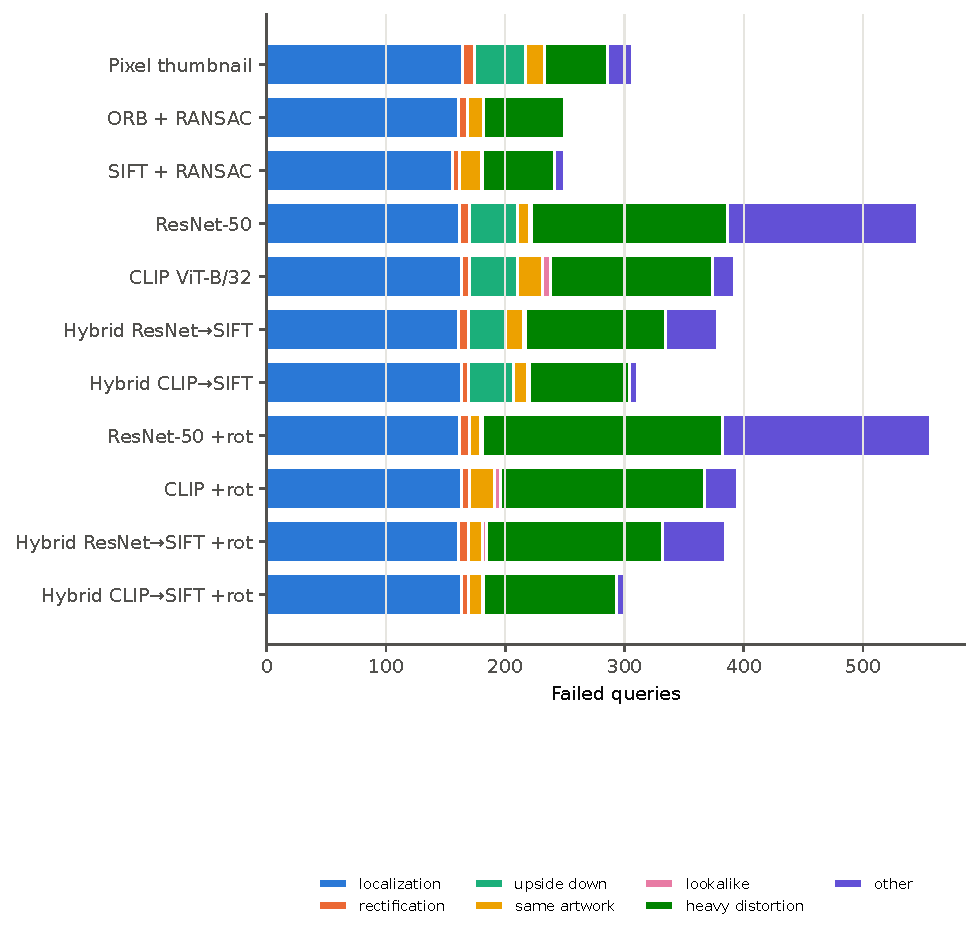
\includegraphics[width=\textwidth]{figures/failure_causes.pdf}
\caption[Failure causes per method]{Failure causes of the strict top-1 errors per method (all severities pooled, \res{main-n-queries} queries per severity).}
\label{fig:failure-causes}
\end{figure}

\begin{figure}[htbp]\centering
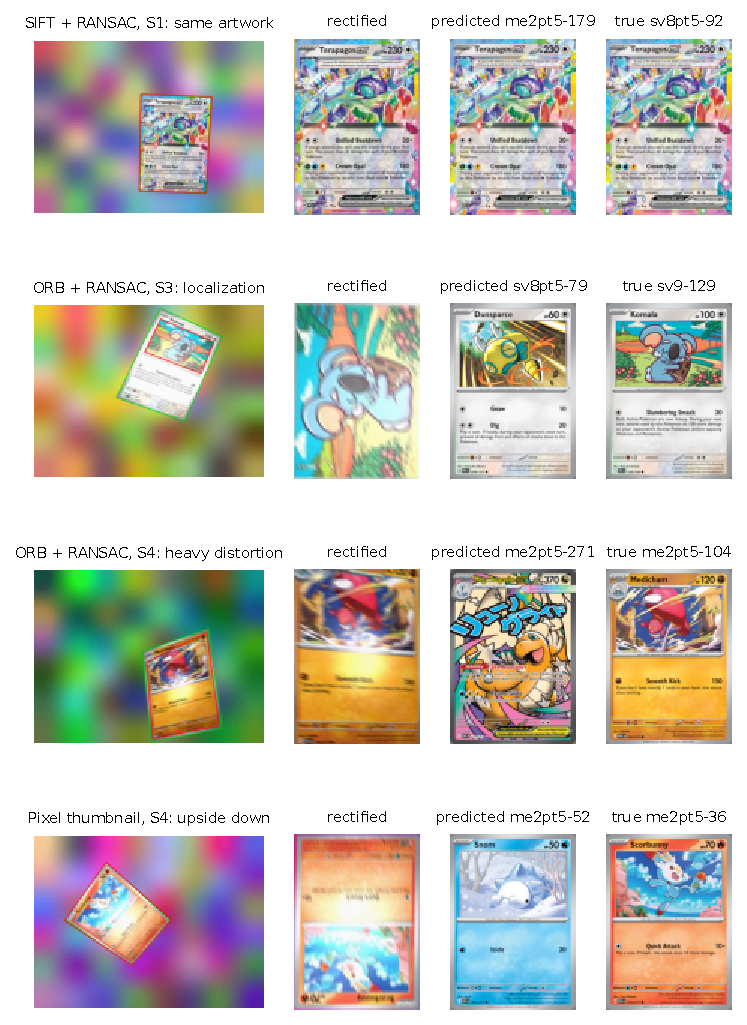
\includegraphics[width=\textwidth,height=0.8\textheight,keepaspectratio]{figures/failure_examples.pdf}
\caption[Failure examples]{Failure examples, one per row: same artwork (SIFT + RANSAC, severity 1); localization (ORB + RANSAC, severity 3); heavy distortion (ORB + RANSAC, severity 4); upside down (Pixel thumbnail, severity 4). Columns: query (green = true outline, red = detected outline), rectified card, predicted reference, true reference.}\label{fig:failure-examples}
\end{figure}


\paragraph{Localisation is the main bottleneck under strong distortion.} Every method shares the same detector and the same queries, so every method had about the same number of localisation failures (\res{fail-orb-localization} for ORB, \res{fail-clip-localization} for CLIP, \res{fail-hybrid_clip_k20-localization} for the CLIP hybrid). Of the \res{fail-orb-total} ORB failures, \res{fail-orb-localization} were localisation failures, and \res{fail-orb-s4} and \res{fail-orb-s5} of all ORB failures happened at severities 4 and 5. When the outline was wrong, identification almost never succeeded: at severity 5, ORB identified \res{orb-s5-top1_given_bad_rect} of the \res{orb-s5-nbadrect} queries with a wrong outline. When the outline was correct, ORB still reached \res{orb-s5-top1_given_rect} at severity 5 and \res{orb-s4-top1_given_rect} at severity 4. So there are two separate problems at high severity: the detector misses the card in most photos, and even a correctly rectified card is often too blurred and noisy for reliable keypoints (\res{fail-orb-heavydistortion} ORB failures are ``heavy distortion'' with a correct outline). Improving the detector (for example with a learned detector) would therefore help more than changing the retrieval method, but would not solve severity 5 alone.

\paragraph{Global embeddings also fail on well-rectified cards.} Apart from reprints, the keypoint methods did not fail when the outline was correct and the distortion moderate (ORB: \res{fail-orb-other} failures of the category ``other''). ResNet-50, in contrast, had \res{fail-resnet-other} failures of the category ``other'' (correct outline, severity 1--3, not a reprint and not a lookalike) and \res{fail-resnet-heavydistortion} ``heavy distortion'' failures, against \res{fail-clip-other} and \res{fail-clip-heavydistortion} for CLIP. A likely reason is that a frozen ImageNet descriptor summarises a card mostly by its overall colour and layout, and many cards of the same energy type and frame design look alike at that level. SIFT re-ranking repairs most of these errors: the CLIP hybrid had only \res{fail-hybrid_clip_k20-other} ``other'' failures and the ResNet hybrid \res{fail-hybrid_resnet_k20-other}.

\paragraph{Reprints and lookalikes are rare.} At severities 1 and 2, all strict errors of ORB and SIFT were reprint confusions (Section~\ref{sec:res-main}). This is expected: a reprint has the same artwork, and the only visible differences are the set symbol, the set code and the collector number in the bottom strip, which are only a few pixels tall at $500\times700$. The lenient metric shows that the method found the right \emph{artwork} in every one of these cases. A dedicated second stage that reads the collector number (OCR at higher resolution, as already done for the language) could separate them. Lookalike errors (same name, different artwork) did not occur at all for ORB and SIFT and were rare for the embeddings (\res{fail-clip-lookalike} for CLIP, \res{fail-resnet-lookalike} for ResNet-50, \res{fail-hybrid_clip_k20-lookalike} for the CLIP hybrid), so the different versions of the same Pok\'emon are distinguished well.

\paragraph{Upside-down cards.} Rotation-sensitive methods failed on cards that the warp returned upside down: \res{fail-pixel-upsidedown} times for the pixel baseline, \res{fail-resnet-upsidedown} for ResNet-50 and \res{fail-clip-upsidedown} for CLIP, all at the severities with large rotations, while ORB and SIFT had none because they are rotation invariant. The +rot variant removed these failures completely, but, as shown in Section~\ref{sec:res-main}, did not raise the overall accuracy, because other failures took their place.

\section{How realistic are the synthetic results?}
\label{sec:disc-synthetic}

The pixel-thumbnail baseline, which compares $32\times44$ grey thumbnails, identified \res{pixel-s1-top1} of the queries at severity 1 and \res{pixel-s3-top1} at severity 3, more than ResNet-50 (\res{resnet-s3-top1}) and CLIP (\res{clip-s3-top1}) alone at severity 3. Such a simple method can only work this well because each synthetic query is rendered from the \emph{same} scan that is in the database: once the card is correctly rectified, query and reference are almost the same image up to blur, noise and lighting. A real photo of a physical card differs from the scan also in printing, colour reproduction, surface reflections of holographic cards, sleeves and wear. The real photos saved in the application confirm this: there the pixel baseline identified only \res{app-pixel-hits} of the \res{app-reid-n} cards, while SIFT, ORB, CLIP and the CLIP hybrid identified all of them (Table~\ref{tab:app-reid}). The synthetic benchmark is therefore an optimistic estimate that favours pixel-level similarity; it is reliable for comparing robustness to distortion and for the ranking of the methods that use local features or learned embeddings, but the absolute numbers, and especially the strength of the pixel baseline, do not transfer to real photos.

Two further points limit the comparison across severities: each severity uses a different random set of \res{main-n-queries} cards, and the latencies were measured on a laptop that was running other jobs (including other experiments) at the same time, so they indicate orders of magnitude rather than exact times.

\section{Language, text and the global embeddings}

The cross-language experiment (Section~\ref{sec:res-language-id}) gives a first view of how the method families differ. SIFT + RANSAC was nearly language-independent, which suggests that the artwork keypoints dominate the RANSAC homography and the different text has little influence. CLIP lost accuracy on Spanish and especially Japanese cards, consistent with its embedding being influenced by the text regions; restricting it to the artwork window helped on Japanese cards but the difference is not statistically clear with \res{lang-ja-n} queries. The hybrid recovered most of the gap: the shortlist of CLIP only needs to \emph{contain} the correct card, and SIFT then picks it. Two caveats apply: the Japanese ground truth was matched by artwork similarity, so Japanese cards whose artwork differs from the English print are under-represented; and the cards were shown at severity 2 only.

The same experiment shows the cost side of the trade-off. Exhaustive SIFT took a median of \res{lang-sift-ms}~ms per photo against \res{db-cards} cards, which is too slow for interactive use and grows linearly with the database, whereas the CLIP hybrid needed about \res{lang-hybrid_clip+rot_k20-ms}~ms. The k-sweep on the main benchmark confirms the trade-off (Figure~\ref{fig:ksweep}): the CLIP hybrid reaches close to the accuracy of exhaustive keypoint matching at a fraction of its time, and its cost grows with $k$, not with the size of the database.

\section{What the application shows about real photos}
\label{sec:disc-app}

The \res{app-reid-n} photos saved in the application are too few for statistical conclusions, but they are real photos of real cards, in sleeves, and they point in clear directions.

\paragraph{Identification transfers to real photos.} SIFT, ORB, CLIP and the CLIP hybrid identified every saved photo exactly, including the two Japanese cards. ResNet-50 was again the weakest method: it failed badly on the full-art Morpeko ex, whose whole surface is illustration. With so few photos this is an indication, not proof.

\paragraph{Separate Japanese reference cards are needed for exact identification.} Adding the Japanese \emph{Battle Partners} cards to the application's database made it possible to identify a Japanese copy as the Japanese card (with its own number and price) instead of its English twin. Methods that see the whole card, text included, did this correctly; the artwork-only hybrid, which by design ignores the text, returned the English twin. The two ways of comparing cards therefore answer two different questions: ``which artwork is this?'' (artwork only, language independent) and ``which exact printing is this?'' (whole card, which needs reference scans in every language that should be recognised).

\paragraph{Sleeves move the detected outline, not the answer.} On sleeved cards the detector often locked onto a rectangle slightly inside or outside the real card edge. Identification was robust to this, but the condition estimate is not, because it measures borders, corners and edges at the outline (see below).

\paragraph{Exhaustive SIFT is too slow for the application.} With a median of \res{app-sift-ms}~ms per photo, plain SIFT, which is still the application's default method, makes the user wait many seconds (the screenshot in Figure~\ref{fig:app-screens} shows a similar time), whereas the CLIP hybrid gave the same answers in about \res{app-hybrid_clip+rot_k20-ms}~ms. This supports making the CLIP hybrid the default method. To help the user choose, the application now shows a short description of every method next to the method selector.

\paragraph{The condition estimate does not transfer to real photos yet.} On synthetic damage the estimate was validated (Section~\ref{sec:res-condition}), but on the real photos it produced uniformly low scores and many surface ``defects''. Several causes are visible in the data. (i) Reference mismatch: the front of the Japanese Mega Chandelure was compared with the \emph{English} scan, so the different text counts as damage. (ii) Real-photo conditions: the Japanese Maractus was compared with its own Japanese scan and still produced \res{app-ja-SV9-101-front-ndefects} defects, so reflections of sleeves and holders, the keyboard texture around the card and the inexact outline (above) also generate false defects and penalise edges and corners. (iii) The back side has no clean reference, so it is measured only from its own border colours, and the same back photo appears to have been reused for three cards. The estimate should therefore be presented as experimental. Fixing it requires photos of unsleeved cards on a plain background, as the application already asks for, and a comparison with the true condition of real cards.

\paragraph{Stored language.} The two \emph{Battle Partners} cards were stored with the language ``ja'', because the application now pre-selects Japanese when the matched reference card is Japanese. The Mega Chandelure, which was saved before that change, is still stored as ``en'' although it is a Japanese print; the application does not log whether a stored language came from the OCR classifier or from the user.

\section{Printed language and condition}

The language classifier improved from \res{langclf-v1-test-acc} to \res{langclf-v2-test-acc} on the test split. Version 1 failed in two ways: \res{langclf-v1-test-unknown} photos gave no usable text at low resolution (``unknown''), and \res{langclf-v1-test-falseja} English or Spanish cards were labelled Japanese because the OCR model invented kanji on blurry Latin text. Version 2 addressed both at once (higher resolution for OCR, and only kana count as Japanese evidence), so the separate contribution of each change was not measured. In version 2 almost all remaining errors are ``unknown'' answers rather than wrong languages (\res{langclf-v2-test-unknown} versus \res{langclf-v2-test-wrong}), which is the safer kind of error because the application lets the user correct it. The language-code rule decided only \res{langclf-v2-test-coderule} of the \res{langclf-v2-test-n} test photos, because the OCR model misreads the tiny code box.

For the condition estimate, centering and corner damage are measured reliably on synthetic damage, whereas edge fraying is weak ($\rho=$ \res{cond-rho-edge-fray}): fraying of less than about half a millimetre is only a few pixels wide even at 12 pixels per millimetre. The overall score correlates only moderately with the total damage ($\rho=$ \res{cond-overall}) because the weights that combine the parts are hand-set. The estimate is useful to flag visible problems, but it is not a substitute for a professional grade.
